\documentclass[conference]{IEEEtran}
\IEEEoverridecommandlockouts
% The preceding line is only needed to identify funding in the first footnote. If that is unneeded, please comment it out.

\usepackage{amsmath,amssymb,amsfonts}
\usepackage{algorithmic}
\usepackage{graphicx}
\usepackage{textcomp}
\usepackage{xcolor}
\usepackage{biblatex}
\addbibresource{final-paper.bib}
\begin{document}

\title{Edges to Handbags}

\author{\IEEEauthorblockN{Zachary Harvey}
\IEEEauthorblockA{\textit{Computer \& Information Science Dept.} \\
\textit{SUNY Polytechnic Institute}\\
Utica, NY, USA \\
harveyz1@sunypoly.edu}
\and
\IEEEauthorblockN{Dr. Michael J. Reale}
\IEEEauthorblockA{\textit{Computer \& Information Science Dept.} \\
\textit{SUNY Polytechnic Institute}\\
Utica, NY, USA \\
realemj@sunypoly.edu}
}

\maketitle

\begin{abstract}
In this resarch, we are trying to build solid photo-like images of handbags from 2-D outline drawings of representative bags.
We build a pix2pix U-Net model to help accomplish this. We show
marginal to good results with this approach; however, we also show some very specific limits regarding the algorithm's inherent bias towards geometric shapes.
\end{abstract}

\begin{IEEEkeywords}
pix2pix, U-NET, outline, drawn
\end{IEEEkeywords}

\section{Introduction}
We are trying to train an algorithm to build pictures of handbags from 2-D line drawings. This proves to be challenging because we have very little input in these drawings, specifically in terms of design details, material choices, and other elements that actually could affect handbag shape. Further, by starting with a 2-D line drawing, we are completely ignoring shadow, arguaby one of the most important elements for determining shape from a 2-D image. The approach taken to successfully train the algorithm could be applied to a wide variety of objects, not just handbags. It would also enable designers to filter through ideas quickly, going from sketchbook to object rapidly to determine if a design is visually appealing or not. We are using pix2pix and U-Net to accomplish this task.

\section{Related Work}
We are taking the core architecture from pix2pix \cite{imagetoimage}. The pix2pix
authors were able to achieve promising results with their algorithm. However, their approach was
very broad in that they were training with data sets containing numerous object types and we'd like to focus on a singular problem. We, instead, have chosen to focus solely on handbag shapes as our training data sets.  There have been a couple of other
papers discussing this idea of outlines to objects. A group at MIT \cite{6247689} has
had good success with converting basic line drawings to geometric objects. The downside
is this work is really steered towards basic geometric shapes and not any soft organic shapes. While this approach could certainly strengthen generation of objects with natural geometric characteristics, realistically many design items have a much more organic form.
Zheng and Zhu \cite{zheng2022deep} have also showed other ways of reconstructing a 3D object from a line drawing with decent success; however this, too, also looks to be geared towards mostly rigid-bodied objects.


\section{Method}
We use a U-Net pix2pix architecture built in TensorFlow and Keras. The code for the
architecture was taken from the pix2pix tutorial on TensorFlow's website \cite{pix2pix}.
We have eight steps down. Each step is a sequential layer with a 2D convolution and an optional
batch normalization which is only on the first layer. Then the output of the convolution is
pushed through a leaky relu. On the up side we have seven layers. Each layer is a sequential layer
with a 2D convolution transposed. We always apply a batch normalization. A dropout of 0.5 is
applied to the first three layers. The output is then pushed through a relu. We
insert skip connections. This creates our generator as seen in \ref{fig:generator}.
\par
The discriminator is much smaller as we can see in figure \ref{fig:discriminator}. We take in the image generated by the generator. We run
it through three layers. Each layer is a sequential layer with a 2D convolution to an optional
normalization which is then passed through a leaky relu. The normalization is passed through
the last two layers. Once we're through those layers we pad out our data with zeros. We then pass it
through another 2D convolution, followed by a batch normalization. Then we have a
leaky relu to more padding and finally another 2D convolution.
By using this method we were hoping to achieve handbag generation at a consistent and simple level.
We will use this as a jumping off point to get more complex handbag shapes.
\subsection{Data}
The data set is comprised of 138,767 single images files. Each image has a width of 512 pixels and a
height of 256 pixels. Each single image file contains two images paired together. The left side image is
the outline of our handbag at size 256 by 256. The right side image is a side profile of the
actual bag at size 256 by 256.


\section{Experiments}
We ran through the normal data set from the pix2pix \cite{imagetoimage} paper. We had mixed
results here.
\begin{figure}[h]
  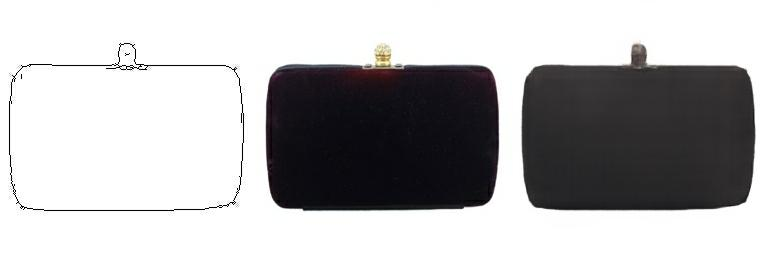
\includegraphics[width=0.5\textwidth]{./image_dump_39000.jpg}
  \caption{\label{fig:handbag39} Handbag after 39,000 steps}
  \centering
\end{figure}
The bag in figure \ref{fig:handbag39} had good results after 39,000 steps. The shape looks correct, as does the color, although the hardware has lost its gold coloring. The larger handbag example in figure
\ref{fig:missing-data}, however, shows some problems. It appears that the algorithm is inventing the bottom shape of the bag
as the input drawing is missing that information.
\begin{figure}[h]
  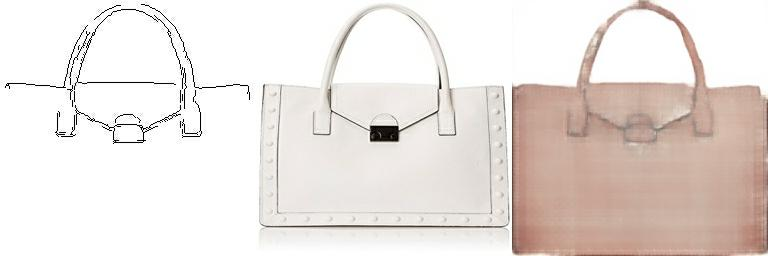
\includegraphics[width=0.5\textwidth]{./bad_result.jpg}
  \caption{\label{fig:missing-data} Input is missing data.}
  \centering
\end{figure}
To explore this theory, we decided to use non-square handbag examples through the algorithm. We were hoping to see how the algorithm handled these instances.
This would help lead us to determine how it was handling input with missing data.
\begin{figure}[h]
  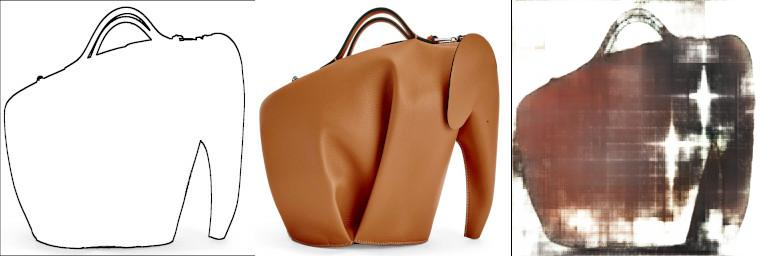
\includegraphics[width=0.5\textwidth]{./bad_elephant_33000.jpg}
  \caption{\label{fig:loewe} Loewe Elephant bag after 33,000 steps}
  \centering
\end{figure}
This bag designed and manufactured by Loewe is an elephant shape. We took a side profile and built an outline with GIMP. The exampe in figure \ref{fig:loewe} shows the image generated after
33,000 steps. It appears the algorithm prefers to build square or rectanglar bags. It seems to ignore the open space between the bag and the trunk of the elephant. 
\begin{figure}[h]
  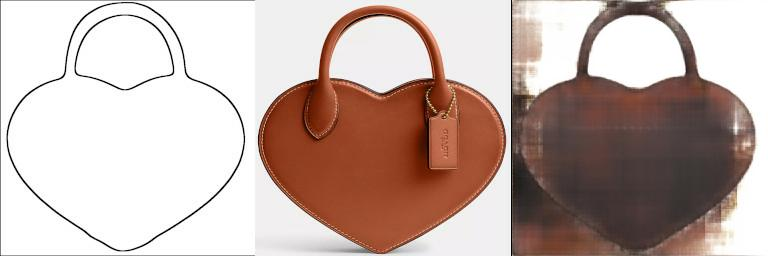
\includegraphics[width=0.5\textwidth]{./heart_33000.jpg}
  \caption{\label{fig:coach} Coachs Heart bag after 33,000 steps}
  \centering
\end{figure}
The Coach Heart bag in figure \ref{fig:coach} also suggests that the algorithm favors square bags. 

\begin{figure}[h]
  \includegraphics[width=0.5\textwidth]{./imagetoimage_output.png}
  \caption{\label{fig:imagetoimage} Sample output from image to image paper \cite{imagetoimage}}
  \centering
\end{figure}
However the output Isola and Zhu \cite{imagetoimage} published appears to have cleaned up a lot of these results and shows success with slightly more rounded organic shapes.
This suggests that maybe we did not train for long enough.

\section{Conclusion}
Our results show that there is a larger body of resarch to be done before precise object generation from 2-D line drawings can be accomplished. Though the handbag examples
that have been generated here are not as detailed or precise as desired, the ideas are promising. With further research, we could provide greater detail, including color and material choices. If we added stable diffusion to our architecture,
we could get richer input from users and further hone our output.


\begin{figure}[p]
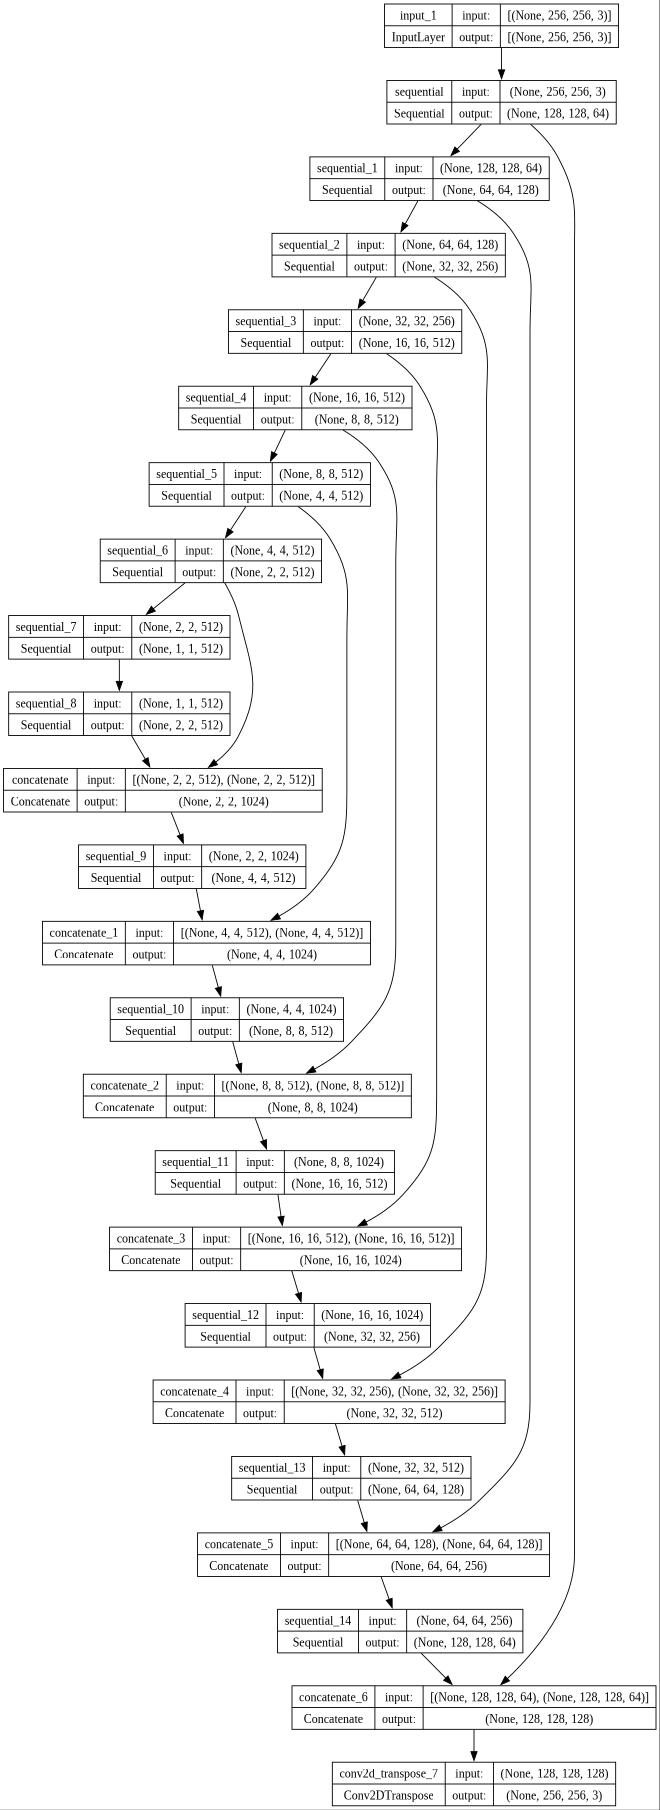
\includegraphics[scale=0.25]{./generator.jpg}
  \caption{\label{fig:generator} This is our diagram of the generator.}
\centering
\end{figure}

\begin{figure}[p]
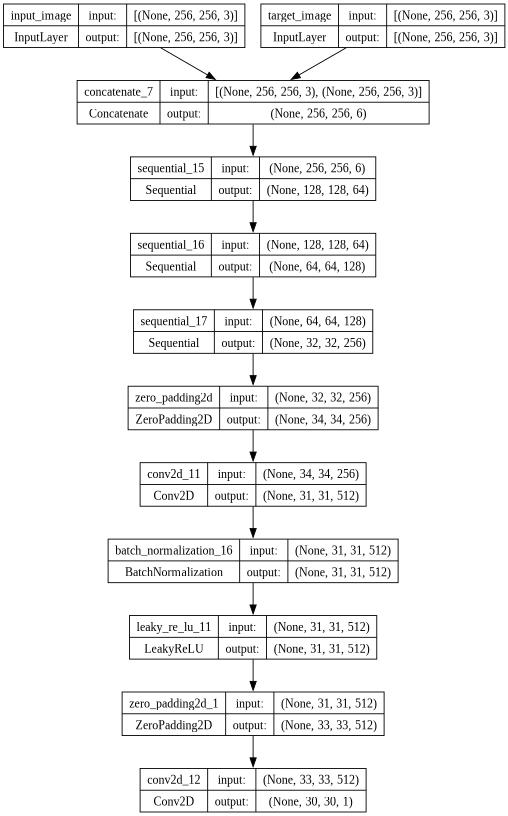
\includegraphics[width=0.38\textwidth]{./discriminator.jpg}
  \caption{\label{fig:discriminator} This is our diagram of the discriminator.}
\centering
\end{figure}
\printbibliography
\end{document}
